% ===================== ANALISIS DE RESULTADOS =====================
\section{Análisis de Resultados}
\label{sec:analisis}

Este capítulo discute el impacto del diseño de profundización por Perforación Horizontal Dirigida (PHD) sobre la operación del salmueroducto de BRINSA S.A., evaluando los riesgos de succión, sedimentación, acumulación de gases y resistencia mecánica.

% ─────────────────────────────────────────────────────────────────────────────
\subsection{Evaluación del Impacto en la Presión de Succión (Km8 y Km17)}
\label{ssec:analisis_succion}

El principal requerimiento del cliente consiste en determinar si la profundización del trazado en el Humedal Arrieros (Km 16.5) genera pérdidas de carga significativas que comprometan la presión de succión en la estación Km8, cuya puesta en marcha está prevista para finales de este año.

Los resultados numéricos (Tabla~\ref{tab:resumen_resultados}) demuestran que el incremento neto de pérdidas de presión dinámica es de tan solo \SI{0.65}{\kilo\pascal} (\SI{0.007}{bar}) para la línea de salmuera y \SI{0.45}{\kilo\pascal} (\SI{0.004}{bar}) para la línea de condensado. Este incremento porcentual de \SI{1.69}{\percent} y \SI{1.80}{\percent}, respectivamente, se considera despreciable desde la perspectiva del diseño de sistemas de bombeo. 

Físicamente, esto ocurre debido a dos factores:
1. La longitud física adicional por la geometría inclinada del túnel de perforación es de únicamente \SI{2.26}{\meter} en comparación con el trazado superficial horizontal original de \SI{450.00}{\meter}.
2. La diferencia de elevación neta entre el punto de lanzamiento y llegada es favorable (el punto de llegada se encuentra \SI{0.79}{\meter} por debajo del punto de lanzamiento). En estado estacionario de flujo continuo, bajo la condición de sifón lleno, las cargas de elevación vertical se cancelan mutuamente de acuerdo con la ecuación de Bernoulli.

Por lo tanto, se concluye cuantitativamente que \textbf{no existe una afectación significativa en la presión de succión de las estaciones Km8 y Km17} bajo condiciones de operación nominal estable.

% ─────────────────────────────────────────────────────────────────────────────
\subsection{Riesgo de Sedimentación y Obstrucción en el Sifón Invertido}
\label{ssec:analisis_sedimentacion}

Al profundizar la tubería por debajo del humedal se genera una configuración física de sifón invertido. La salmuera transportada se encuentra en estado de saturación (\SI{26}{\percent} p/p de \text{NaCl}), lo que implica un riesgo inherente de precipitación de cristales de sal ante disminuciones de temperatura o detenciones del flujo. Asimismo, el arrastre de sólidos menores (arenas o impurezas) es común en este tipo de redes de conducción.

Para evitar la acumulación de sólidos y la consecuente reducción del área de flujo en el fondo plano de la perforación (cota \SI{2542.75}{m.s.n.m.}), la velocidad del fluido debe superar la velocidad crítica de autolimpieza ($v_c$). De acuerdo con criterios de la *Hydraulic Institute (HI)* y heurísticas de transporte de pulpas y salmueras, la velocidad mínima de arrastre de sólidos finos se sitúa en el rango de \SI{0.9}{\meter\per\second} a \SI{1.2}{\meter\per\second}.

Dado que la velocidad de flujo calculada para la salmuera es de \SI{1.60}{\meter\per\second} a condiciones nominales, el sistema opera en un margen seguro de autolimpieza. Sin embargo, si el caudal volumétrico desciende por debajo de \SI{169}{\cubic\meter\per\hour} (equivalente a \SI{47}{\liter\per\second} o una velocidad de \SI{0.90}{\meter\per\second}), se activa un riesgo alto de sedimentación en el fondo de la PHD.

% ─────────────────────────────────────────────────────────────────────────────
\subsection{Riesgo de Acumulación de Gases en Puntos Altos}
\label{ssec:analisis_gases}

La geometría de sifón invertido de la PHD crea dos crestas o puntos altos locales de transición en el plano de perfil 202609-BRI-SE-CIV-PL-001-RB.pdf: el punto de lanzamiento a la abscisa K0+000 (cota \SI{2558.35}{m.s.n.m.}) y el punto de llegada a la abscisa K0+450 (cota \SI{2557.56}{m.s.n.m.}). 

Durante el llenado de la línea, el aire atrapado migrará naturalmente hacia estos picos altos. De igual manera, la liberación de gases disueltos en el condensado o la salmuera debido a fluctuaciones de presión y temperatura se acumulará en estas secciones. La formación de bolsas de aire en las crestas genera:
1. Bloqueo por aire (*air binding*), el cual incrementa significativamente la resistencia hidráulica aparente, reduciendo el caudal de operación.
2. Transitorios de presión severos (golpes de ariete) durante arranques y paradas debido a la compresión súbita de las bolsas de gas.

% ─────────────────────────────────────────────────────────────────────────────
\subsection{Distinción entre Presión Operativa Dinámica y Presión Estática de Parada}
\label{ssec:analisis_dinamico_vs_estatico}

El diseño mecánico del tramo enterrado por Perforación Horizontal Dirigida (PHD) debe distinguir dos estados físicos distintos: la condición de **operación dinámica** y la condición de **parada en vaso comunicante**.

En operación dinámica, el fluido circula impulsado por las estaciones de bombeo y la presión en cualquier punto obedece al balance de energía de Bernoulli generalizado:

\begin{equation}
    P_2 = P_1 + \rho g (z_1 - z_2) + \Delta P_{\text{bombas}} - \Delta P_{\text{fricción}}
    \label{eq:bernoulli_generalizado}
\end{equation}

En esta condición existen pérdidas por fricción a lo largo de la conducción, por lo que la presión en el fondo del sifón puede ser significativamente menor que la presión estática de referencia. El modelo dinámico desarrollado en AFT Fathom para la línea de salmuera confirma que, para caudales entre 250 y 300 m³/h, la presión operativa en el tramo del Km~16.5 se sitúa en el rango de aproximadamente 2.9 a 6.0 bar (Tabla~\ref{tab:presion_operativa_vs_parada}).

En parada total sin válvulas de corte, el sistema se comporta como un vaso comunicante. Al anularse el flujo, las pérdidas por fricción desaparecen y la acción de las bombas cesa. La presión en el fondo del sifón queda gobernada únicamente por la columna hidrostática desde el tanque de quiebre atmosférico:

\begin{equation}
    P_{\text{fondo, parada}} = \rho g (z_{\text{tanque}} - z_{\text{fondo}})
    \label{eq:presion_parada}
\end{equation}

Para la salmuera saturada, esta presión alcanza \SI{13.59}{bar} en el fondo del PHD, valor que supera la capacidad de la tubería SDR~13.6 (PN12.7) y justifica el rediseño a SDR~11 (PN16).

La Tabla~\ref{tab:presion_operativa_vs_parada} contrasta ambas condiciones y evidencia por qué la presión de parada es el caso gobernante para el diseño mecánico de la tubería.

\begin{table}[htbp]
    \centering
    \caption{Comparación entre presión operativa dinámica y presión estática de parada en el fondo del PHD (salmuera saturada).}
    \label{tab:presion_operativa_vs_parada}
    \small
    \setcounter{itemcount}{0}
    \begin{tabularx}{\textwidth}{@{}N>{\raggedright\arraybackslash}p{3.8cm}>{\centering\arraybackslash}p{2.2cm}>{\raggedright\arraybackslash}p{3.5cm}>{\raggedright\arraybackslash}X@{}}
        \toprule
        \multicolumn{1}{c}{\textbf{Item}} & \textbf{Condición} & \textbf{Presión [bar]} & \textbf{Gobernante para} & \textbf{Observación} \\
        \midrule
        & Operación dinámica (Fathom, 250--300 m³/h) & 2.9 -- 6.0 & Diseño de bombas, NPSH y succión & Incluye pérdidas por fricción \\
        & Parada en vaso comunicante & 13.59 & Diseño mecánico de tubería (SDR) & Peor caso; independiente del caudal \\
        \bottomrule
    \end{tabularx}
\end{table}

La independencia de la presión estática de parada respecto al caudal es un resultado crítico: el bajo flujo operativo actual o futuro no atenúa el sobreesfuerzo mecánico del SDR~13.6 en salmuera. Por ello, la selección del espesor de pared debe basarse en la condición estática de parada, mientras que el análisis dinámico valida que las pérdidas por fricción en operación no comprometen el punto de succión de las estaciones de bombeo.

% ─────────────────────────────────────────────────────────────────────────────
\subsection{Evaluación Mecánica e Integridad Estructural de la Tubería HDPE}
\label{ssec:analisis_mecanico}

La integridad mecánica del tramo enterrado por Perforación Horizontal Dirigida (PHD) a la cota clave de fondo de \SI{2542.75}{m.s.n.m.} depende de la presión interna total a la que se expone el material. Si el sistema opera sin válvulas de aislamiento intermedias (comportamiento global), el fondo del sifón en el Km~16.5 se encuentra presurizado por la columna hidrostática acumulada desde el tanque de quiebre atmosférico de salmuera ($2658.24\ \text{m.s.n.m.}$) o desde la estación de bombeo de condensado ($2597.00\ \text{m.s.n.m.}$, provisional). La cabeza estática resultante es de \SI{115.49}{\meter} para salmuera y \SI{54.25}{\meter} para condensado.

La presión de diseño total en el punto más bajo ($P_{\text{diseño}}$) se calcula de acuerdo con la Ecuación~\ref{eq:pfondo}, sumando la presión dinámica local de entrada en superficie ($P_{\text{din, sup}}$) y el efecto hidrostático global:

\begin{equation}
    P_{\text{diseño}} = P_{\text{din, sup}} + \rho g \cdot dH_{\text{global}}
    \label{eq:pfondo}
\end{equation}

Para el circuito de salmuera saturada ($\rho = \SI{1200}{\kilogram\per\cubic\meter}$), la columna hidrostática global genera una presión estática en parada de \SI{13.59}{bar}. Para el circuito de condensados ($\rho = \SI{1000}{\kilogram\per\cubic\meter}$), esta presión es de \SI{5.32}{bar}. En la Figura~\ref{fig:perfil_presiones_estaticas} se presenta la distribución de presiones estáticas a lo largo del tramo local para los escenarios de operación global y local aislado, contrastándolos con los límites nominales de las tuberías SDR~13.6 (PN12.7) y SDR~11 (PN16).

\begin{figure}[htbp]
    \centering
    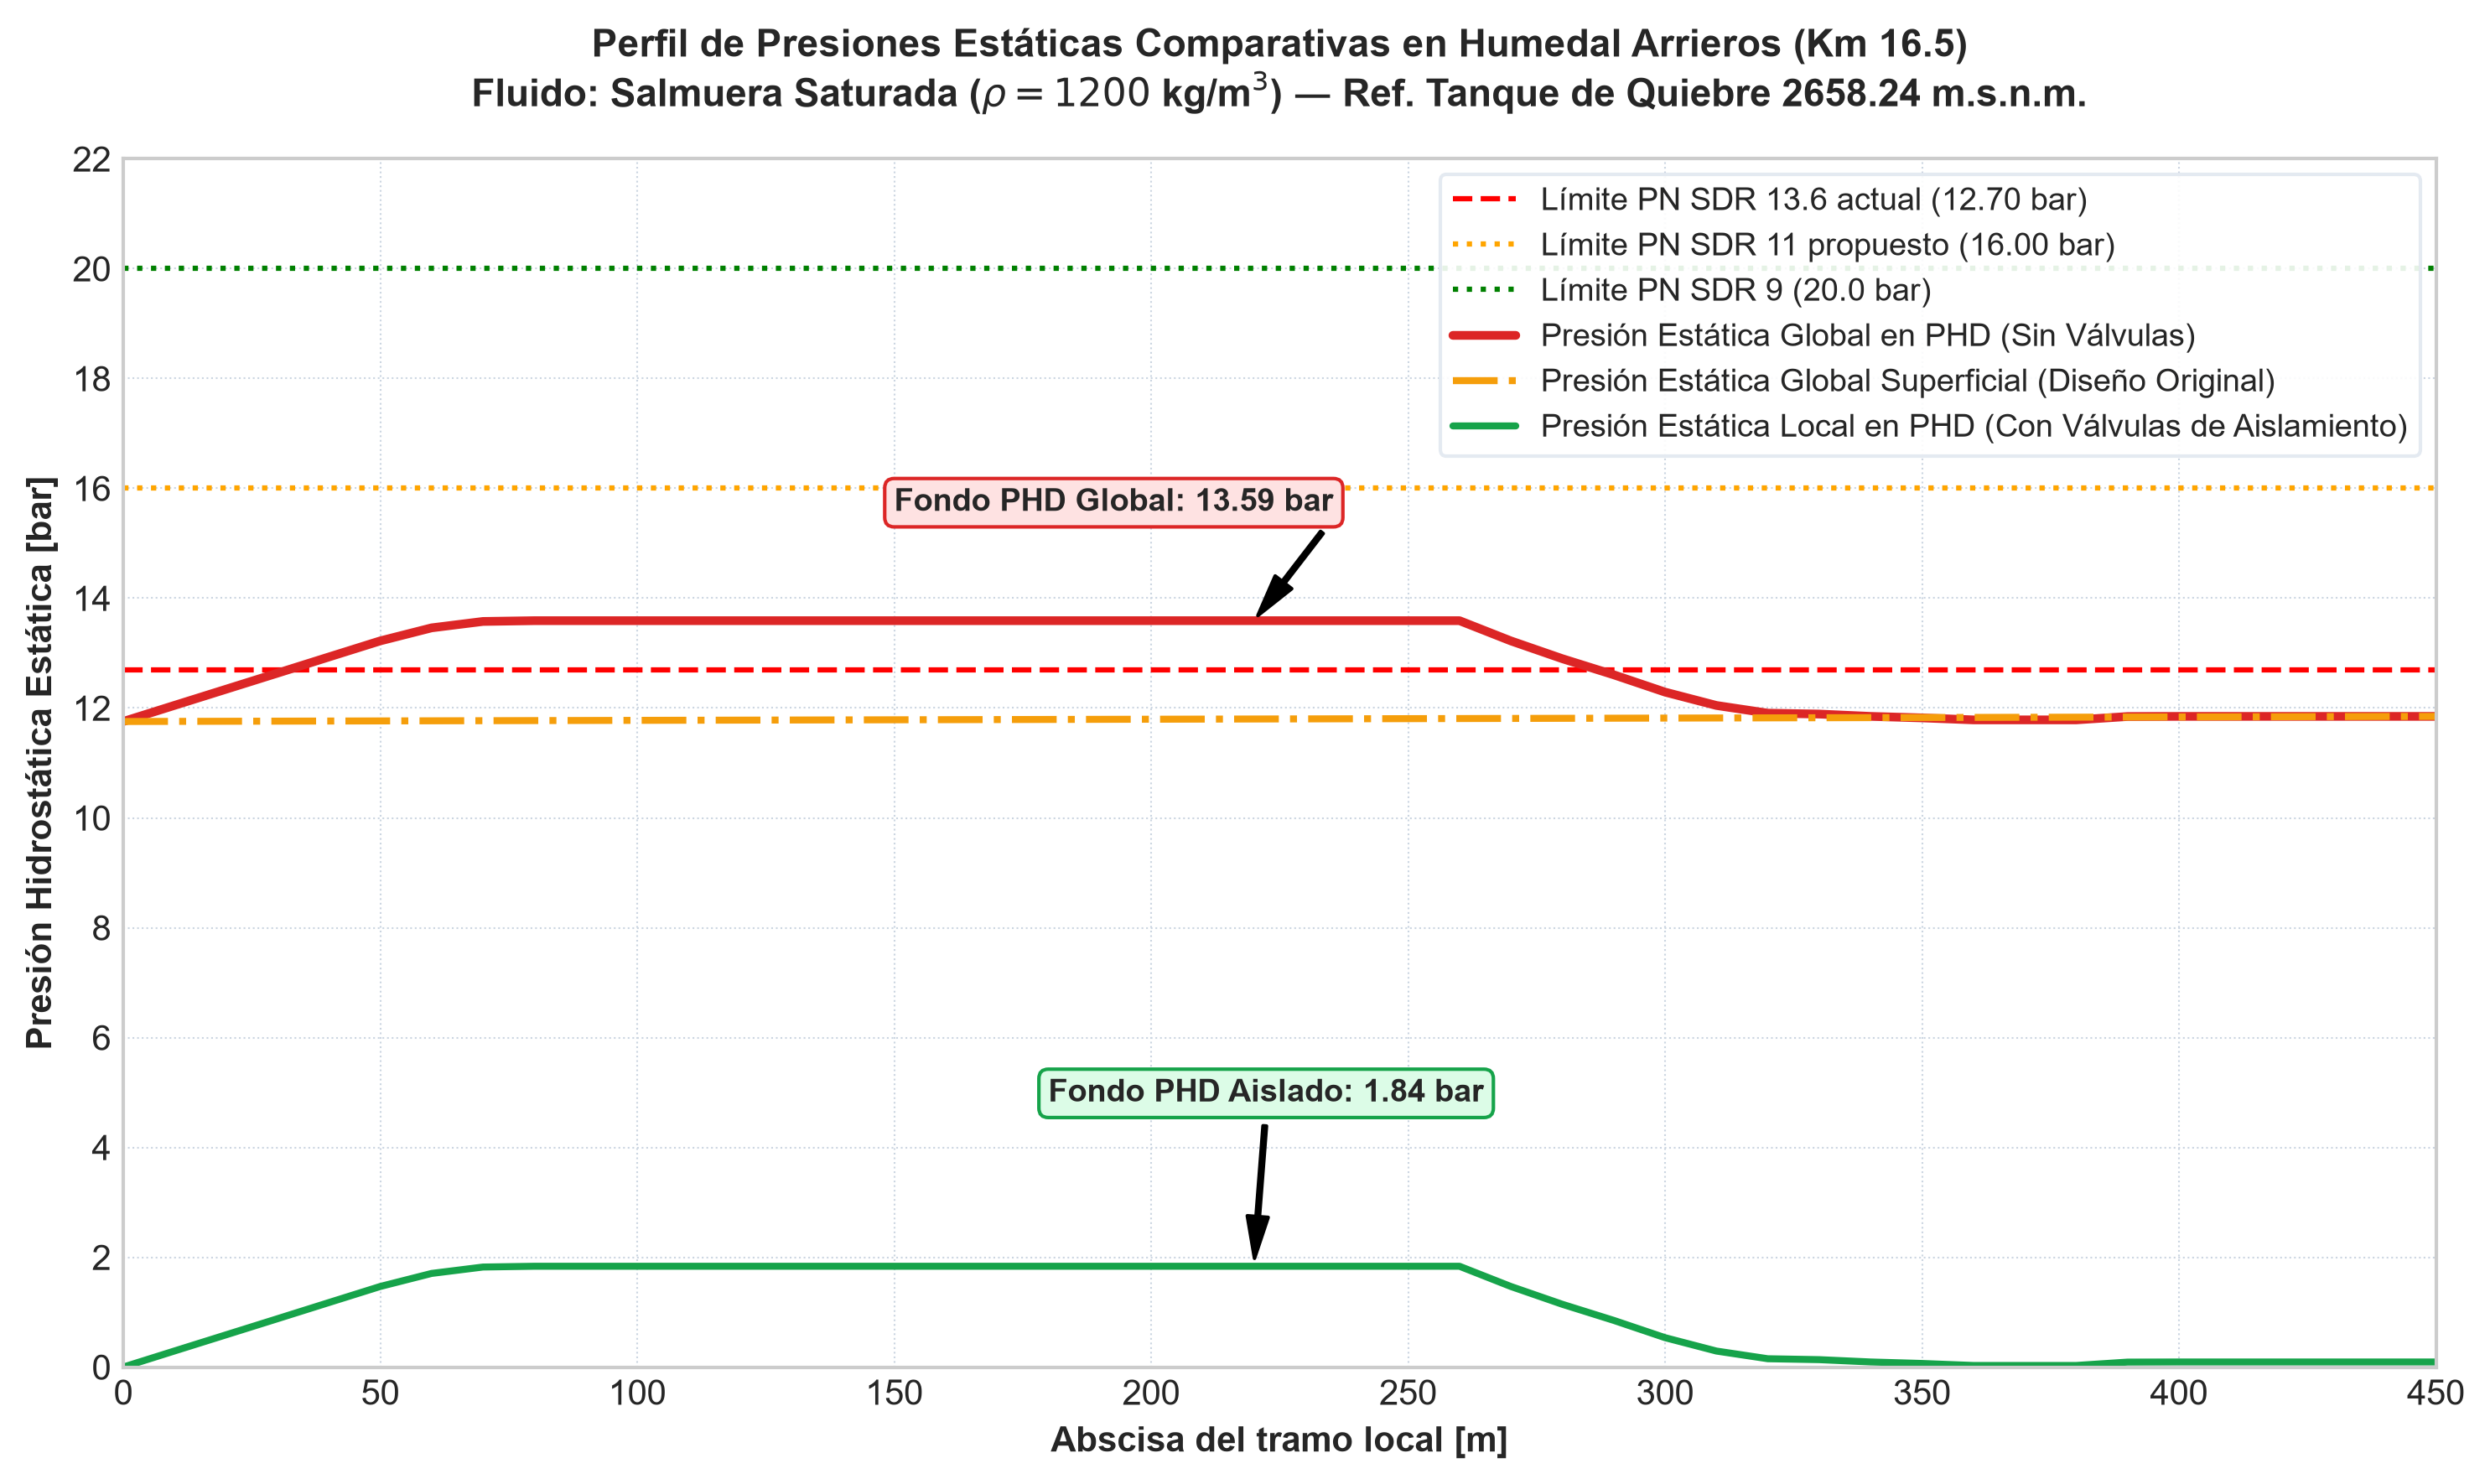
\includegraphics[width=0.90\textwidth]{assets/perfil_presiones.png}
    \caption{Perfil de presiones estáticas hidrostáticas comparativas en el tramo Km 16.5 (Humedal Arrieros) para el escenario global y local aislado en salmuera saturada.}
    \label{fig:perfil_presiones_estaticas}
\end{figure}

Para evaluar formalmente el espesor de pared mínimo requerido ($t_{\text{mín}}$) bajo los estándares de diseño mecánico aplicables, se implementan las ecuaciones de esfuerzo límite. Según la norma ISO 4427, el espesor mínimo para tuberías termoplásticas se calcula a partir de la Resistencia Mínima Requerida (MRS) y el coeficiente de diseño ($C=1.25$ para agua/fluidos industriales a \SI{20}{\celsius}) mediante la Ecuación~\ref{eq:t_iso}:

\begin{equation}
    t_{\text{mín, ISO}} = \frac{P_{\text{diseño}} \cdot OD}{2 \cdot \left( \frac{MRS}{C} \right) + P_{\text{diseño}}}
    \label{eq:t_iso}
\end{equation}

Por su parte, el código de tuberías de proceso ASME B31.3 (Sección A304.1.2) define el espesor mínimo en función del esfuerzo hidrostático de diseño ($HDS = \SI{5.0}{\mega\pascal}$ para PE100 a condiciones industriales, equivalente a un factor de seguridad del \SI{50}{\percent} sobre el MRS) a través de la Ecuación~\ref{eq:t_asme}:

\begin{equation}
    t_{\text{mín, ASME}} = \frac{P_{\text{diseño}} \cdot OD}{2 \cdot HDS + P_{\text{diseño}}}
    \label{eq:t_asme}
\end{equation}

La Tabla~\ref{tab:espesores_sdr_disenio} compara la integridad mecánica de la tubería actual SDR~13.6 y la propuesta SDR~11 para ambos circuitos de proceso en el escenario global, utilizando un diámetro exterior base $OD = \SI{315.0}{\mm}$.

\begin{table}[htbp]
    \centering
    \caption{Comparación de integridad mecánica entre SDR 13.6 actual y SDR 11 propuesto.}
    \label{tab:espesores_sdr_disenio}
    \small
    \setcounter{itemcount}{0}
    \begin{tabularx}{\textwidth}{@{}N>{\raggedright\arraybackslash}Xcc>{\raggedright\arraybackslash}X>{\raggedright\arraybackslash}X@{}}
        \toprule
        \multicolumn{1}{c}{\textbf{Item}} & \textbf{Servicio / fluido} & \textbf{$P_{\text{est}}$} & \textbf{SDR actual / prop.} & \textbf{Presión nominal} & \textbf{Evaluación} \\
        & & \textbf{[bar]} & & \textbf{[bar]} & \\
        \midrule
        & Salmuera saturada (global) & 13.59 & SDR 13.6 & 12.70 & Falla (+7.0\% sobrepresión) \\
        & Salmuera saturada (global) & 13.59 & SDR 11 & 16.00 & Cumple (margen 15.1\%) \\
        & Condensado (agua) (global) & 5.32 & SDR 13.6 & 12.70 & Cumple (margen 58.1\%) \\
        & Condensado (agua) (global) & 5.32 & SDR 11 & 16.00 & Cumple (margen 66.7\%) \\
        \bottomrule
    \end{tabularx}
\end{table}

Con base en la evaluación mecánica estructurada en la Tabla~\ref{tab:espesores_sdr_disenio}, se definen las siguientes conclusiones de diseño técnico:

1. Si no se modifica el sistema y se opera bajo la configuración global (sin válvulas de aislamiento), la tubería actual de SDR 13.6 falla en el circuito de salmuera (sobrepresión del +7.0\% respecto a PN12.7), pero cumple en el circuito de condensado. Por ello, la línea de salmuera se rediseña obligatoriamente a SDR 11 (PN16), la cual cumple con un margen del 15.1\%. El condensado puede mantenerse en SDR 13.6, sujeto a confirmar la cota exacta de la estación de bombeo.

2. La alternativa de optimización técnica e instalación civil más conveniente consiste en la operación de dos válvulas de seccionamiento y aislamiento automáticas en las cámaras de conexión del lanzamiento (Km~16.5) y llegada (Km~16.9) de la PHD. Al activarse el cierre de estas válvulas en paradas del salmueroducto, se confina el sifón de forma aislada, limitando la columna estática al desnivel de la PHD (\SI{15.60}{\meter}). La auditoría de campo del SCADA (Sección~\ref{sec:auditoria}) evidenció que la conducción de salmuera ya cuenta con válvulas de corte de emergencia (\texttt{ESDV-SAL-K17} y \texttt{ESDV-SAL-K8}); por tanto, esta alternativa puede no requerir obra mayor, sujeto a verificar que su posición hidráulica flanquee el cruce del Km~16.5 y que sean de corte estanco (clase VI o ESD), no válvulas de control.

3. Bajo la condición de tramo aislado localmente, la presión máxima en el fondo disminuye a \SI{1.84}{bar} (salmuera) y \SI{1.53}{bar} (condensados). Bajo esta configuración de proceso, tanto la tubería SDR 13.6 como la SDR 11 cumplen con un amplio factor de seguridad, eliminando la necesidad de sobrediseñar el espesor de la red y garantizando la viabilidad del proyecto de profundización sin incurrir en sobrecostos de tuberías especiales.

% ─────────────────────────────────────────────────────────────────────────────
\subsection{Validación con Modelamiento en AFT Fathom}
\label{ssec:validacion_fathom}

Con el fin de verificar la robustez del modelo hidrostático desarrollado en Python para la línea de salmuera, se realizó un modelamiento independiente en el software comercial AFT Fathom. El modelamiento en Fathom consideró la misma geometría de referencia (tanque de quiebre atmosférico a \SI{2658}{m.s.n.m.}, cota de lanzamiento/llegada de la PHD a \SI{2558}{m.s.n.m.} y cota mínima del sifón a \SI{2543}{m.s.n.m.}), fluido salmuera saturada ($\rho = \SI{1200}{\kilogram\per\cubic\meter}$) y condición de flujo estacionario.

La Tabla~\ref{tab:validacion_fathom} presenta la comparación de presiones absolutas/manométricas entre el modelo Fathom y el modelo analítico implementado en este estudio.

\begin{table}[htbp]
    \centering
    \caption{Validación del modelo hidrostático de salmuera con AFT Fathom.}
    \label{tab:validacion_fathom}
    \small
    \setcounter{itemcount}{0}
    \begin{tabularx}{\textwidth}{@{}N>{\raggedright\arraybackslash}Xccc@{}}
        \toprule
        \multicolumn{1}{c}{\textbf{Item}} & \textbf{Punto de evaluación} & \textbf{Fathom [barG]} & \textbf{Modelo Python [bar]} & \textbf{Diferencia} \\
        \midrule
        & Tanque de quiebre (referencia) & 0.00 & 0.00 & --- \\
        & Punto de lanzamiento/llegada PHD & 11.77 & 11.76 & --0.01 bar (--0.1\%) \\
        & Cota más baja del sifón (fondo) & 13.56 & 13.59 & +0.03 bar (+0.2\%) \\
        \bottomrule
    \end{tabularx}
\end{table}

La Figura~\ref{fig:fathom_salmuera} muestra el modelo esquemático generado en AFT Fathom para la línea de salmuera, en el cual se aprecian las elevaciones y las presiones manométricas en los puntos críticos del tramo: tanque de quiebre, lanzamiento/llegada de la PHD y cota más baja del sifón.

\begin{figure}[htbp]
    \centering
    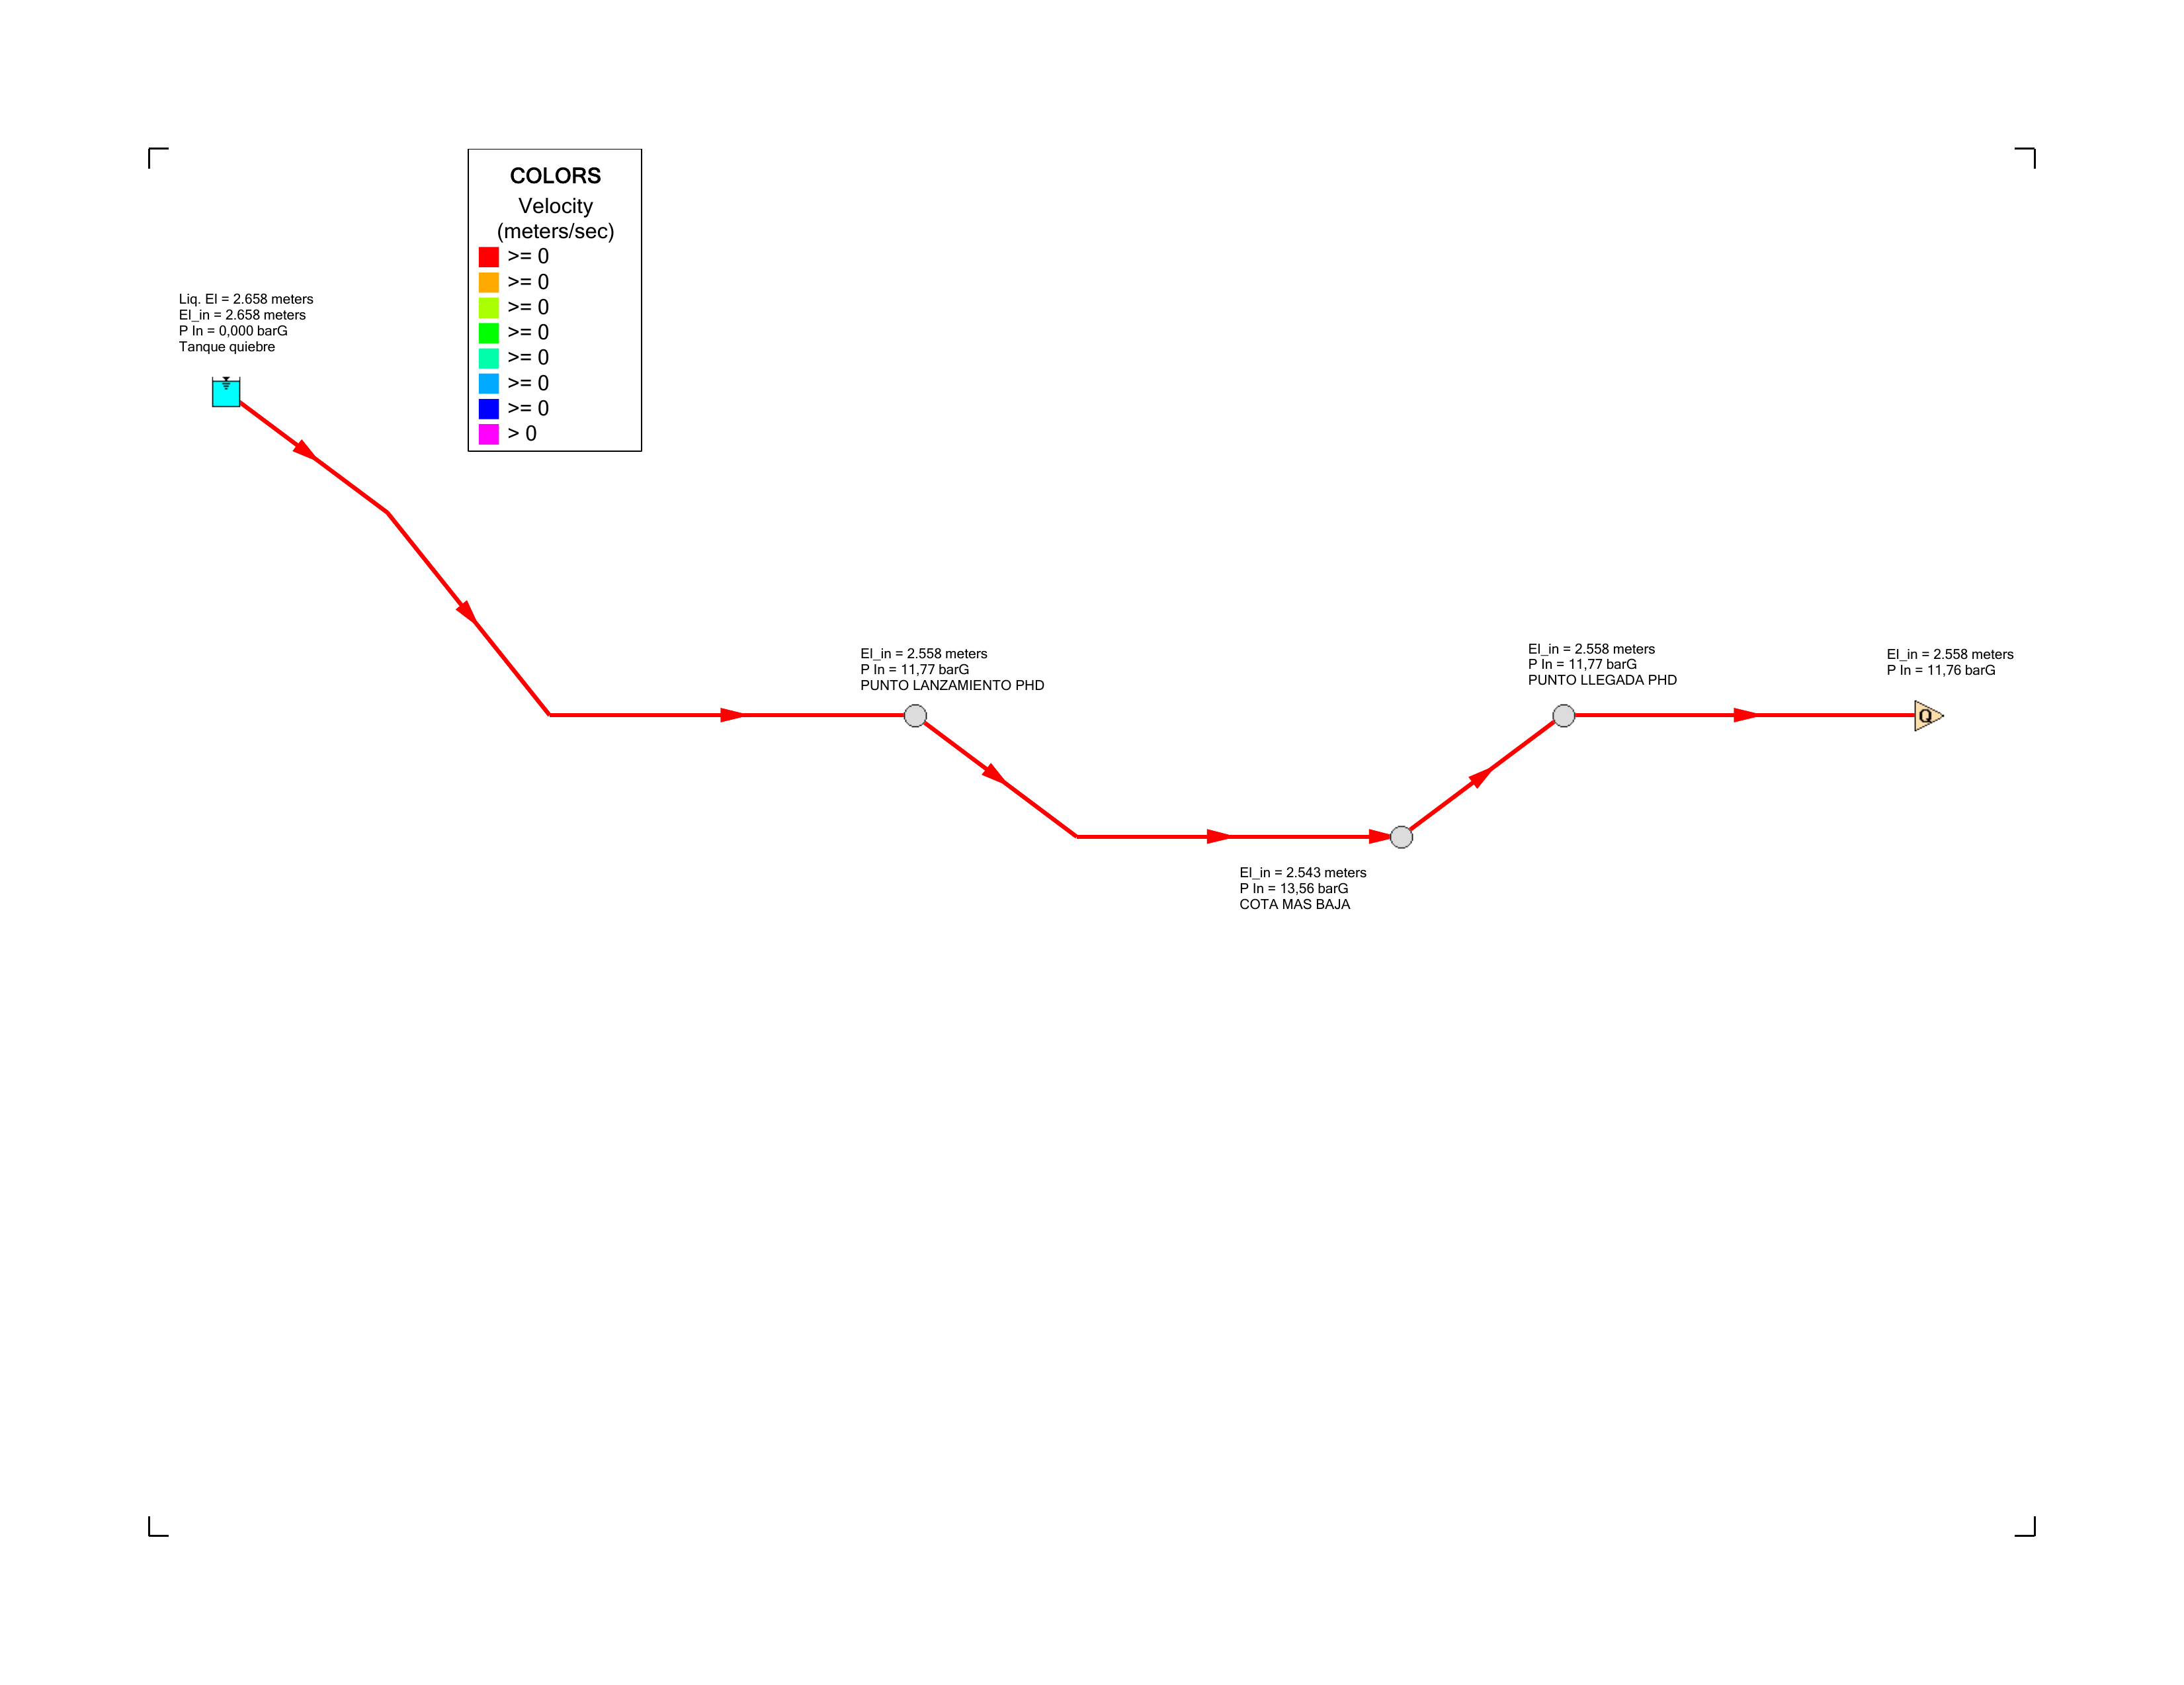
\includegraphics[width=0.95\textwidth]{assets/fathom_salmuera.png}
    \caption{Modelo hidrostático de la línea de salmuera en AFT Fathom (cota de referencia: tanque de quiebre atmosférico a \SI{2658}{m.s.n.m.}).}
    \label{fig:fathom_salmuera}
\end{figure}

La diferencia máxima observada es de únicamente \SI{0.03}{bar} (equivalente a un \SI{0.2}{\percent}) en el punto de fondo del sifón. Esta discrepancia es atribuible a pequeñas diferencias en la precisión de cotas utilizadas (Fathom redondea a metros enteros, mientras que el modelo Python emplea cotas decimales del DXF) y a los métodos numéricos internos del software comercial. Dado que la diferencia es menor al \SI{0.5}{\percent}, se considera que \textbf{el modelo hidrostático desarrollado está validado} y puede utilizarse con confianza como base de diseño mecánico y de selección de SDR para la línea de salmuera.

Adicionalmente, se ejecutó un modelamiento dinámico de la línea de salmuera en estado estacionario para tres condiciones de caudal: 250, 275 y 300 m³/h. El objetivo de este análisis paramétrico fue validar que la pérdida de presión por fricción en el tramo enterrado del Km~16.5 no afecta de manera relevante el punto de succión de las estaciones de bombeo. Aunque el modelo Fathom cubre toda la conducción, el análisis se centró exclusivamente en el tramo de tubería enterrada, identificado en el eje longitudinal (kilómetro multiplicado por 1000) entre las abscisas aproximadas $x = 16\,500\ \text{m}$ y $x = 16\,952\ \text{m}$.

La Tabla~\ref{tab:fathom_dinamico_phd} contrasta, para el mismo tramo PHD y el mismo caudal, la pérdida por fricción obtenida con el modelo analítico implementado en este estudio (Python) y la obtenida con AFT Fathom. La pérdida por fricción de Fathom se calculó descontando de la caída neta el aporte hidrostático neto entre el lanzamiento y la llegada del PHD (0.79 m de desnivel, equivalente a 9.3 kPa para salmuera saturada).

\begin{table}[htbp]
    \centering
    \caption{Comparación de pérdida de presión por fricción en el tramo PHD del Km~16.5: modelo Python vs. AFT Fathom (salmuera saturada).}
    \label{tab:fathom_dinamico_phd}
    \small
    \setcounter{itemcount}{0}
    \begin{tabularx}{\textwidth}{@{}N>{\centering\arraybackslash}X>{\centering\arraybackslash}X>{\centering\arraybackslash}X>{\centering\arraybackslash}X@{}}
        \toprule
        \multicolumn{1}{c}{\textbf{Item}} & \textbf{Caudal} & \textbf{Modelo Python} & \textbf{AFT Fathom} & \textbf{Diferencia} \\
        & \textbf{[m³/h]} & \textbf{[kPa]} & \textbf{[kPa]} & \textbf{[\%]} \\
        \midrule
        & 250 & 28.2 & 32.0 & +13.7 \\
        & 275 & 33.5 & 36.2 & +8.1 \\
        & 300 & 39.2 & 40.6 & +3.5 \\
        \bottomrule
    \end{tabularx}
    \begin{flushleft}
        \footnotesize Modelo Python: tubería HDPE PE100 SDR 11, $L = 452.26$ m, $K = 0.5$, $\epsilon = 1.5\times10^{-6}$ m. Fathom: pérdida por fricción estimada en el tramo $x = 16\,500$--$16\,952$ m.
    \end{flushleft}
\end{table}

La comparación en el mismo tramo y para el mismo caudal muestra diferencias menores al 14\%, con una tendencia decreciente a medida que aumenta el flujo. Estas discrepancias se explican por la selección de rugosidad, el tratamiento de pérdidas menores de entrada y salida del sifón, y el redondeo de cotas en el software comercial. En todos los escenarios evaluados, la pérdida por fricción en el PHD permanece en el orden de decenas de kilopascales, valor despreciable frente a las presiones operativas y de parada del sistema.

La Figura~\ref{fig:fathom_perfil_dinamico} muestra el perfil de presión estática obtenido en Fathom para los tres escenarios de caudal a lo largo de toda la línea de salmuera. Se aprecia que, en operación dinámica, las presiones en el tramo del Km~16.5 se sitúan entre 2.9 y 6.0 bar, muy por debajo de la presión estática de parada de 13.59 bar. Esto confirma que el diseño mecánico de la tubería debe dimensionarse para la condición de parada, no para la operación dinámica.

\begin{figure}[htbp]
    \centering
    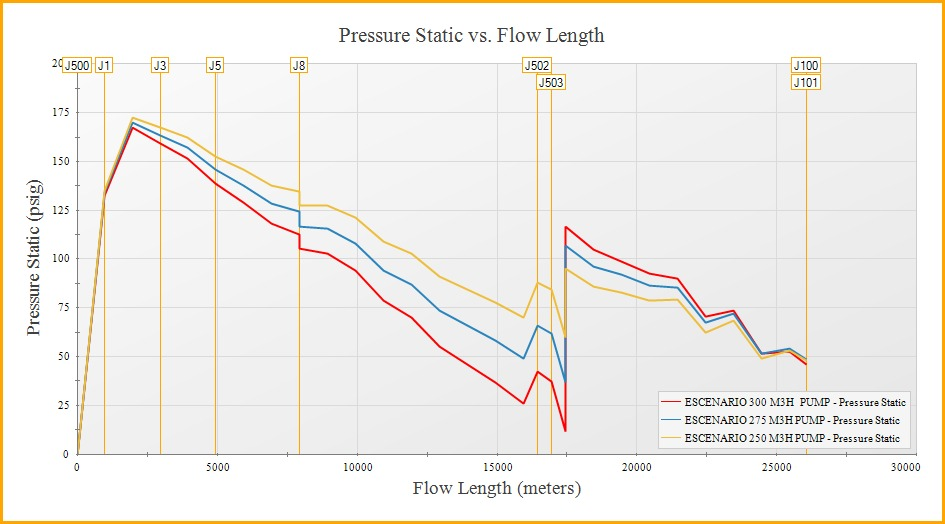
\includegraphics[width=0.95\textwidth]{assets/fathom_perfil_dinamico_original.jpeg}
    \caption{Perfil de presión estática obtenido en AFT Fathom para la línea de salmuera a 250, 275 y 300 m³/h. El eje horizontal corresponde al kilómetro multiplicado por 1000.}
    \label{fig:fathom_perfil_dinamico}
\end{figure}

\begin{figure}[htbp]
    \centering
    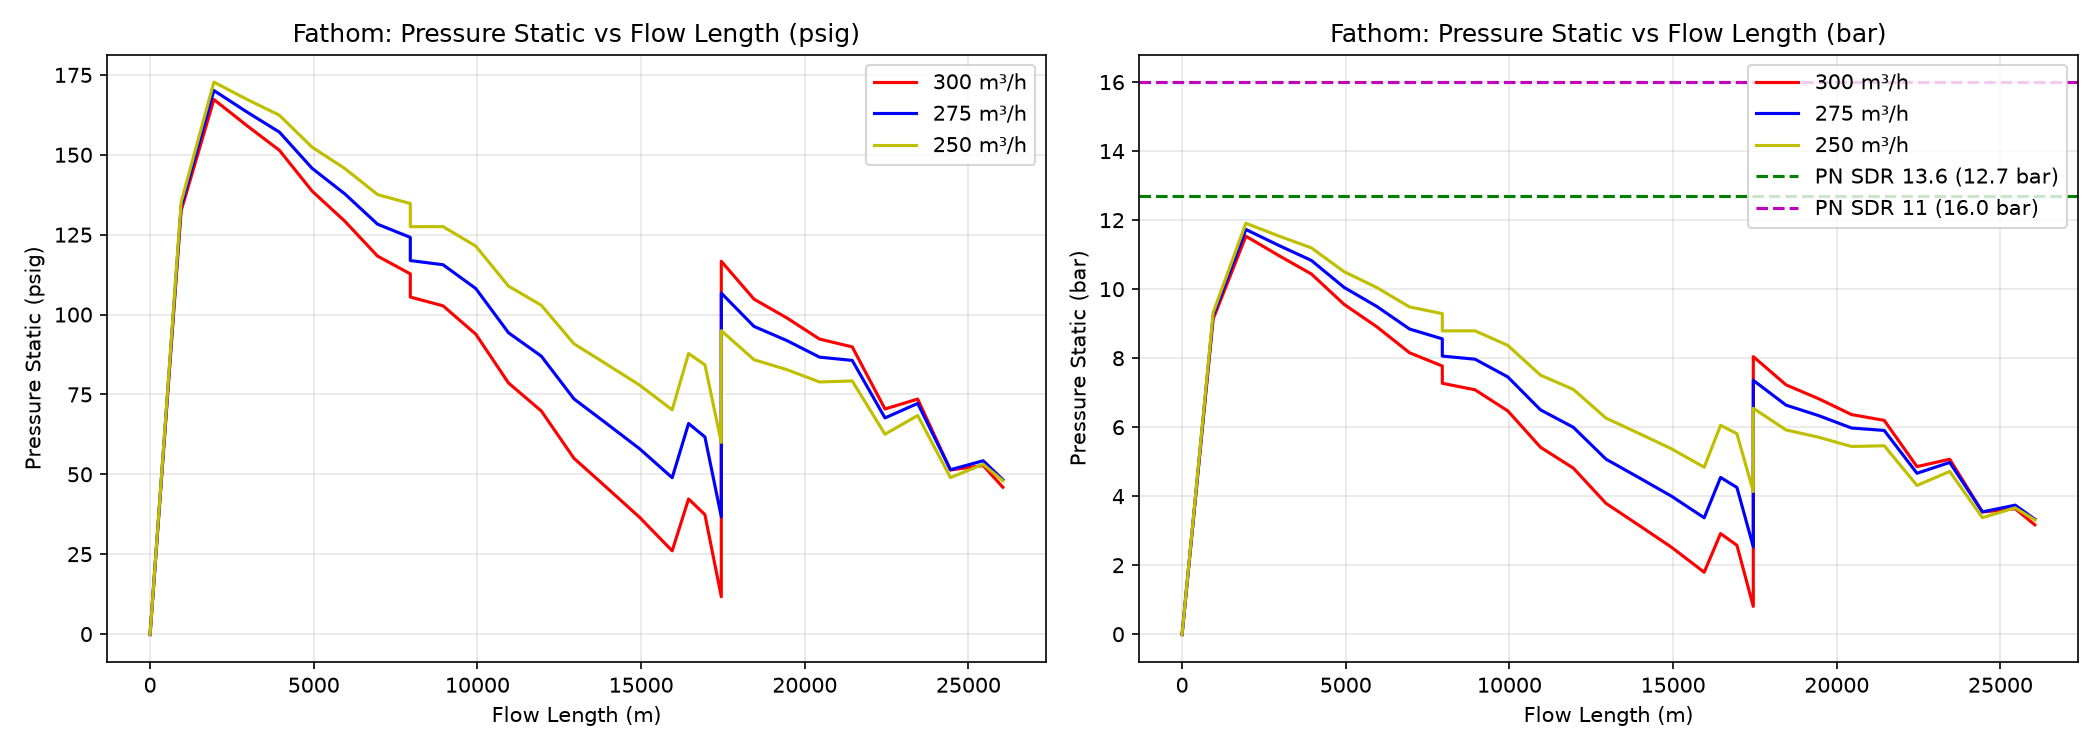
\includegraphics[width=0.95\textwidth]{assets/fathom_perfil_dinamico_reprocesado.png}
    \caption{Perfil de presión estática de Fathom convertido a bar, con indicación de los límites nominales SDR 13.6 (12.7 bar) y SDR 11 (16.0 bar).}
    \label{fig:fathom_perfil_dinamico_reprocesado}
\end{figure}

Se señala como limitación del modelo dinámico de Fathom que no reproduce explícitamente la geometría de sifón invertido del PHD: el perfil de presiones muestra una pendiente descendente continua en el tramo del Km~16.5, sin el valle hidrostático esperado por los 15.6 m de desnivel hasta el fondo del sifón. Por tanto, el modelo Fathom se utiliza en este estudio únicamente para validar el orden de magnitud de las pérdidas por fricción dinámica y el comportamiento operativo de la línea, no para cuantificar la presión estática de parada en el fondo del sifón, la cual continúa calculándose mediante la hidrostática del vaso comunicante.

% ─────────────────────────────────────────────────────────────────────────────
\subsection{Efectos de la Zona Inundable sobre la Estabilidad de la Tubería Enterrada}
\label{ssec:analisis_inundable}

El archivo \texttt{PERFILPROYECTO.dxf} identifica el cruce PHD del Km~16.5 dentro de una zona inundable, con cotas de terreno entre \SI{2560}{m.s.n.m.} y \SI{2563}{m.s.n.m.} El fondo del sifón se proyecta a \SI{2542.75}{m.s.n.m.}, lo que representa una profundización de aproximadamente \SI{15.6}{\meter} bajo la superficie del humedal. Esta condición geotécnica introduce efectos que deben considerarse en paralelo al análisis hidráulico y mecánico, particularmente en lo relativo a flotación, erosión de cobertura y estabilidad durante la construcción.

\textbf{1. Empuje hidrostático vertical (flotación).} Cuando el suelo alrededor de la tubería se satura durante eventos de inundación o por elevación del manto freático, el agua ejerce un empuje de Arquímedes sobre el tubo. Para una tubería de HDPE PE100 con diámetro exterior $OD = \SI{315}{\mm}$, la fuerza de levantamiento teórica por metro lineal es:

\begin{equation}
    U = \frac{\pi}{4} D_{ext}^{2} \cdot \gamma_w \approx \SI{0.77}{\kilo\newton\per\meter}
    \label{eq:empuje_vertical}
\end{equation}

Con una cobertura de \SI{15.6}{\meter} de suelo saturado ($\gamma' \approx \SI{10}{\kilo\newton\per\cubic\meter}$) sobre el tubo, el peso efectivo del prisma de suelo confinado al ancho del diámetro es del orden de \SI{49}{\kilo\newton\per\meter}, valor muy superior al empuje de flotación. Por tanto, \textbf{en el tramo horizontal profundo del PHD la cobertura natural ancla ampliamente el tubo} y no se requiere lastre permanente gravitacional, \textit{siempre que se mantenga la cobertura y exista contacto efectivo suelo-tubo}.

El caso crítico de flotación ocurre cuando el tubo está vacío (mantenimiento, pruebas hidrostáticas, drenajes o paradas prolongadas) y el espacio anular no transmite el peso del suelo. En esas condiciones, el peso propio del tubo (\SI{20.2}{\kilogram\per\meter} para SDR~13.6 y \SI{24.5}{\kilogram\per\meter} para SDR~11) es inferior al empuje de \SI{77.9}{\kilogram\per\meter} y el tubo tiende a flotar. Se recomienda verificar formalmente este estado límite con factor de seguridad mínimo \mbox{$FS \geq 1.25$--$1.50$} contra flotación.

\textbf{2. Reducción de la carga efectiva del suelo.} Las tuberías de HDPE son flexibles y dependen de la interacción suelo-tubería para soportar cargas externas. En suelo saturado, el peso efectivo del relleno sobre la clave del tubo disminuye, reduciendo el confinamiento lateral y vertical. Esto puede incrementar la deflexión vertical del anillo; la deflexión permisible para tuberías de PE suele limitarse al \SI{7.5}{\percent} del diámetro (ASTM~D3034 / Handbook of PE Pipe). En el tramo profundo del cruce, la gran cobertura compensa la reducción de peso unitario, pero la calidad del relleno anular y su compactación son determinantes.

\textbf{3. Erosión y socavación.} El riesgo geotécnico principal no es la flotación en profundidad, sino la \textbf{pérdida de cobertura por erosión superficial} en las zonas de entrada y salida del PHD y en tramos de transición donde la cobertura disminuye. Durante eventos de inundación, el flujo sobre el humedal puede socavar o lavar el relleno, exponiendo sectores del tubo y generando puntos de apoyo desiguales que concentran tensiones locales y aumentan el riesgo de fatiga en el HDPE.

\textbf{4. Tecnologías de protección aplicables.} Con base en la práctica internacional para cruces de tuberías en humedales y zonas inundables (AWWA~M55, PPI~Handbook of PE Pipe, ASTM~F1962, ASCE~MOP~108), se identifican las siguientes medidas de mitigación:

\textbf{1. Lastre por peso.} Collarines o sillas de hormigón pre-fabricadas (``set-on'' / ``bolt-on'') con almohadilla de fieltro o EPDM para no dañar el tubo; bolsas de geotextil rellenas de arena o grava local. Para tubo expuesto, un collarín de \SI{500}{\kilogram} sumergido puede espaciarse aproximadamente cada \SI{5}{\meter}--\SI{6}{\meter}, aunque en instalaciones marinas AWWA~M55 recomienda espaciamientos más cercanos (\SI{1.5}{\meter}--\SI{3.0}{\meter}) por control de flecha y aire.

\textbf{2. Anclaje mecánico.} Anclajes helicoidales (CHANCE, TorcSill) o anclas de percusión (Platipus, MANTA~RAY) unidos al tubo con correas de poliéster y accesorios en acero inoxidable 304/316. Útiles en transiciones con cobertura reducida o suelos blandos, con factor de seguridad $\geq 2.0$ en capacidad última del ancla.

\textbf{3. Relleno anular estructural.} Inyección del anular PHD con lechada cemento-bentonita o CLSM (Controlled Low Strength Material) mediante tubería tremie. Esto garantiza contacto suelo-tubo, aporta peso sumergido, reduce asentamientos diferenciales y corta flujos preferenciales de agua. Requiere controlar la presión de inyección para no distorsionar el tubo.

\textbf{4. Protección contra erosión superficial.} Geotextil no tejido de polipropileno (mín. \SI{8}{\kilo\newton\per\meter} de tracción) como separador/filtro; capa de rip-rap sobre geotextil; gaviones o colchacriado (Reno mattresses) para alta energía; geoceldas rellenas de grava/vegetación para estabilización de taludes. La protección debe extenderse aguas arriba y aguas abajo del cruce (típicamente \SI{10}{\meter}--\SI{20}{\meter}, o 3--5 veces el ancho del cauce según estudio hidráulico) y clavarse en el fondo para evitar socavación por debajo.

\textbf{5. Control de flotación durante la instalación PHD.} ``Water ballasting'', es decir, llenado parcial de la tubería con agua limpia durante el halado para lograr flotabilidad neutra, reducir la tensión de tracción y evitar colapso por presión externa del lodo de perforación. Se requiere cabeza estanca y control riguroso del nivel interno por debajo del lodo de perforación (ASTM~F1962).

\textbf{6. Recomendación preliminar para el proyecto.} Dada la gran cobertura del tramo profundo ($\sim$\SI{15.6}{\meter}), \textbf{no se requiere lastre permanente en el tramo horizontal del PHD}, siempre que el relleno anular garantice transferencia de carga del suelo al tubo. El diseño debe concentrarse en:

\begin{enumerate}
    \item Especificar relleno anular con lechada cemento-bentonita o CLSM, y verificar la transferencia de peso del suelo.
    \item Aplicar water ballasting durante el tiro PHD y verificar tensión de halado según ASTM~F1962 / PPI Handbook.
    \item Proteger las zonas de entrada/salida y transición con geotextil + rip-rap o gaviones, extendiendo la protección al menos \SI{10}{\meter}--\SI{20}{\meter} aguas arriba y aguas abajo del cruce.
    \item Instalar collarines de hormigón o anclas en tramos de cobertura reducida ($<\SI{1.5}{\meter}$) o expuestos por erosión, y verificar flotación con tubo vacío.
    \item Especificar ventosas automáticas de triple efecto en puntos altos del sifón y drenajes en el punto bajo para facilitar llenado, vaciado y mantenimiento.
\end{enumerate}

La interacción suelo-tubería en zona inundable constituye una verificación geotécnica obligatoria para la ingeniería de detalle, complementaria al diseño hidráulico y mecánico presentado en este informe. Se requiere un estudio geotécnico e hidrológico del cruce para confirmar niveles freáticos, erodibilidad, capacidad portante y profundidad de socavación de diseño.

